\section{Access control} The BI-DBS portal uses role-based access control. In the third chapter I have designed the roles system and described their permissions. With the use of that system I have implemented the regulation of displaying the components and controlling access by roles and also verification of users authorization for accessing components and making requests.

\subsection{Role-based access control} Vue Router is first of all responsible of displaying the components by given path. However it has multiple other features which I have used for my implementation.\\
Firstly it allows dynamically setting of different parameters in meta object, you can see the example of a component configuration and meta object in Figure 4.8.\\

\noindent \textbf{Meta parameters for the component:}

\begin{itemize}
    \item \emph{requireAuth:} This flag simply tells if the authorization is required for accessing the component.
    \item \emph{allowAccess:} This flag specifies the role that has permssion to that component.
    \item \emph{sidebar:} Sidebar parameter tells the name of the configuration for navigation side bar items.
    \item \emph{showSideBar:} This attribute is defining whether the navigation side bar should be displayed.
    \item \emph{showTopBar:} This flag is used for the configuration of the top navigation bar and it makes clear if that bar should be displayed for that component.
\end{itemize}

\begin{lstlisting}[language=Octave, caption=The example of component configuration in Router]
{
    path: '/administration',
    component: ImportSemester,
    meta: {
    requireAuth: true,
        allowAccess: Role.GUARANTOR,
        sidebar: 'administration',
        showSideBar: true,
        showTopBar: true
    }
}
\end{lstlisting}

\noindent First two meta parameters are used for the access control, which is implemented as Router configuration. Router allows to set a set of functionalities before each routing which I have used for the verification of a users access to the component. This validation is presented on Listing 4.5.


\begin{lstlisting}[language=Octave, caption=The example of component configuration in Router]
export function configureGuard() {
    Router.beforeEach((to, from, next) => {
        if (to.meta.requireAuth === false) {
            next()
        } else if(verifyAccess(to, from)){
            next()
        }
    })
}

function verifyAccess(to: RouteLocationNormalized, from: RouteLocationNormalized) {
    const userStore = useUserStore()
    userStore.setPreviousPage(from.path)
        
    if (!userStore.isLoggedIn) {
        login()
    } else {
        if (userStore.user.exp_time < new Date()) {
            refreshToken()
        } else {
            return verifyRole(to)
        }
    }
    return false
}

function verifyRole(to: RouteLocationNormalized) {
    if (to.meta.allowAccess == undefined || hasRole(to.meta.allowAccess as Role)) {
        return true
    } else {
        Router.push('/error403')
        return false
    }
}
\end{lstlisting}

\noindent Firstly this configuration checks the users's authorization status if the authorization is required for the component. Secondly it verifies that a user does have the permission to access this component. In a case user is trying to access some component directly without having an access they will be redirected to the error page with an option to get to the previous page, the error component is shown in Figure 4.5.

\begin{figure}[hp]
\centering
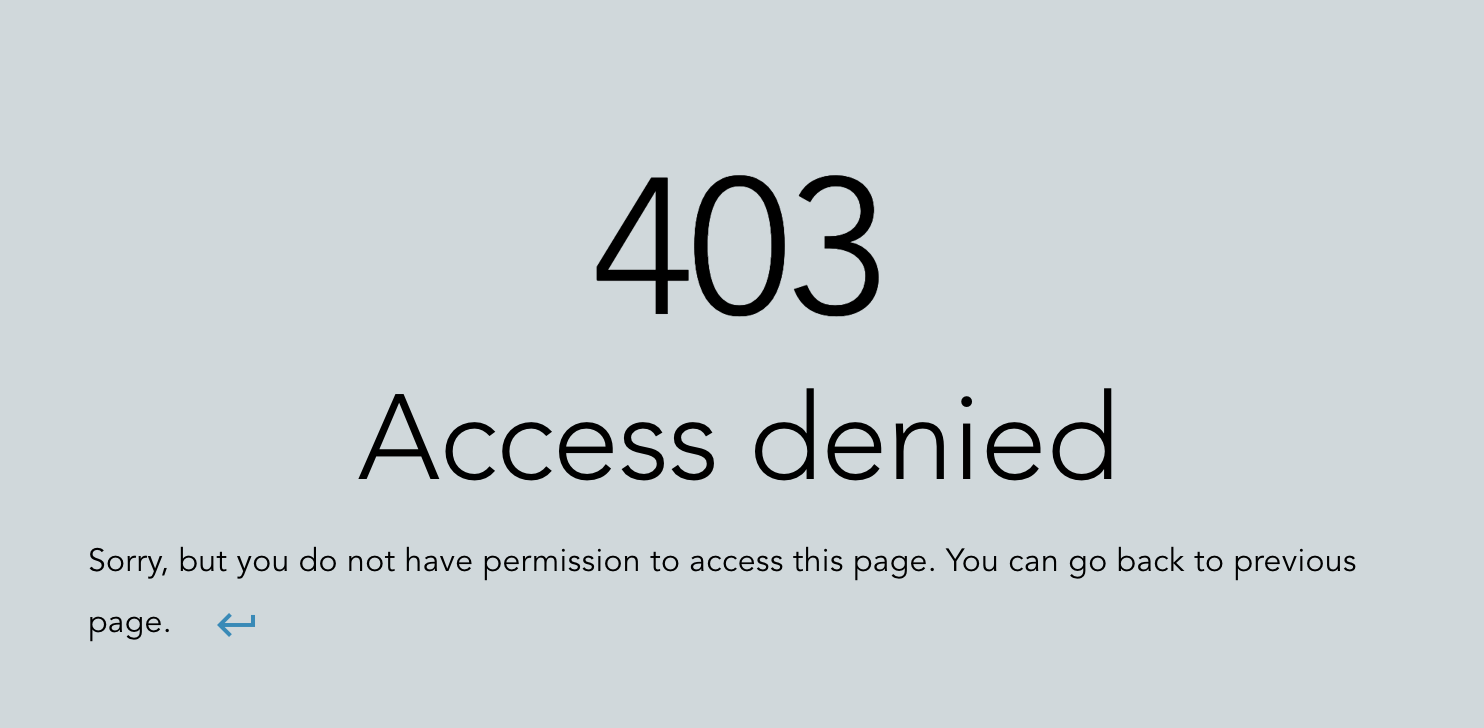
\includegraphics[scale=0.5]{../png/access_denied.png}
\caption{Refresh access token}
\end{figure}



\paragraph*{Display control of components.} Another example of role-based access control benefits and usage is using it for the display-control of UI components. A developer can easily control displaying of any component by setting the required role for it and using the \texttt{hasRole()} function shown on listing 4.6. The code listing 4.7. shows exactly the case like that. In the top navigation bar configuragion I have set the required role for displaying the administration component and used a filter for displaying only the components user has an access to.

\begin{lstlisting}[language=Octave, caption=The example of component configuration in Router]
export function hasRole(role: RoleTOBE) : boolean {
    switch (role) {
        case RoleTOBE.GUARANTOR:
            return isGuarantor()
        case RoleTOBE.TEACHER:
            return isStudent()
        case RoleTOBE.STUDENT:
            return isTeacher()
        default:
            return false
    }
}
\end{lstlisting}


\begin{lstlisting}[language=Octave, caption=The example of component configuration in Router]
function useTopBarConfig() {
    return computed(() => {
        const { t } = useI18n()
        return {
            tabs: [
                { name: t('base.home'), path: '/' },
                { name: t('admin.administration'), path: '/administration' , allowAccess: Role.GUARANTOR },
            ].filter(item => item.allowAccess == undefined || hasRole(item.allowAccess))
        }
    })
}
\end{lstlisting}



\noindent The implementation of regulating accesses and displaying components is clear, flexible and easy to use. It is possible possible due to the role-based access control, which allows simplified permissions management. Moreover such system decreases the risk of data leaking and provides a good visibility over the application.


\

\subsection{Authentication control for requests} Another important validation is verification of an access for making requests to avoid pointless calling of backend services when the user is not authorized or the access token has expired. Especially in the case when the access token has expired we need to detect it and execute the refresh process.\\
In 4.3.2.2 I have provided a code listing 4.3 of configuration the Axios interceptors for the request. That configuration contains a \texttt{verifyAccess()} function which makes sure user is authorized before making the request. That function is illustrated in the listing 4.8.\\


\begin{lstlisting}[language=Octave, caption=TS example]
function verifyAccess() : Promise<string>{
    return new Promise((resolve, reject) => {
        const userStore = useUserStore()
        
        if(!userStore.isLoggedIn){
            reject('Unauthorized')
        } else if (userStore.user.exp_time < new Date()) {
            Auth.refreshToken({
                access_token: userStore.token
            }).then((response) => {
                processResponseToken(response.data.access_token)
                resolve(userStore.token)
            }).catch(() => {
                reject('Unauthorized')
            })
        } else {
            resolve(userStore.token)
        }
    })
}
\end{lstlisting}
